\pagebreak

\section{SOP: Barcode printing}
\label{section:sop_barcode}

ALIIAS generates a set of barcodes during at pseudonymization. These barcodes are saved in the folder displayed on the 'PseudoID' panel, when finishing a pseudonymization transaction (see Step 6 in section \ref{section:sop_aliias} fro details) in separate \path{.png} files and a single \path{.pdf} file.

The latter file contains all barcodes (Fig \ref{fig:barcodes}) in a single file, on separated pages. The researcher can use any PDF-viewer (e.g. with Adobe acrobat Reader) to open the file and print all barcodes with the default printing feature of the software.

\todo{integrate some Z02-SOPs with detailed \newline instructions about neuroendocrine stuff here?}

\begin{figure}[H]
\centering
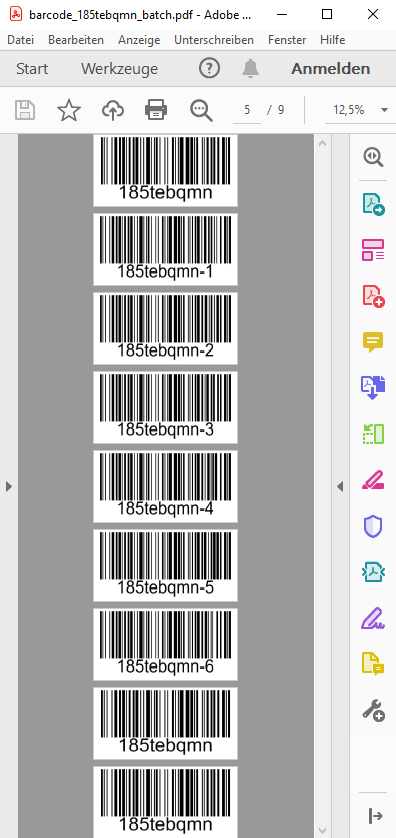
\includegraphics[width=0.4\textwidth]{docs/fig/09_barcodes.PNG}
\caption{The pdf file containing the 9 barcodes, to be used for labelling the saliva tubes (numbered from 1-6), the tubes genetic assessment (without extra number) and the 'participant box' (without extra number) in SFB289.}
\label{fig:barcodes}
\end{figure}